% 2001 年春季京蒙皖卷第 11 题：正方体平面展开图
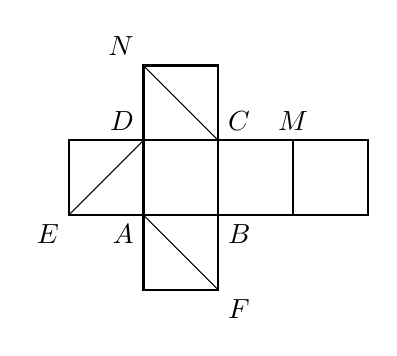
\begin{tikzpicture}[scale=0.95]
  \coordinate (A) at (0,0);
  \coordinate (B) at (1,0);
  \coordinate (C) at (1,1);
  \coordinate (D) at (0,1);
  \coordinate (E) at (-1,0);
  \coordinate (EL) at (-1,1);
  \coordinate (N) at (0,2);
  \coordinate (NT) at (1,2);
  \coordinate (F) at (1,-1);
  \coordinate (FB) at (0,-1);
  \coordinate (M) at (2,1);
  \coordinate (MR) at (2,0);
  \coordinate (RR) at (3,1);
  \coordinate (RRL) at (3,0);

  \draw[thick] (A)--(B)--(C)--(D)--cycle;
  \draw[thick] (E)--(A)--(D)--(EL)--cycle;
  \draw[thick] (D)--(C)--(NT)--(N)--cycle;
  \draw[thick] (A)--(B)--(F)--(FB)--cycle;
  \draw[thick] (C)--(M)--(MR)--(B)--cycle;
  \draw[thick] (M)--(RR)--(RRL)--(MR);
  \draw (E)--(D) (N)--(C) (A)--(F);

  \node[above left] at (N) {$N$};
  \node[above left] at (D) {$D$};
  \node[above right] at (C) {$C$};
  \node[above] at (M) {$M$};
  \node[below left] at (E) {$E$};
  \node[below left] at (A) {$A$};
  \node[below right] at (B) {$B$};
  \node[below right] at (F) {$F$};
\end{tikzpicture}
